\chapter{Conclusion}
brief of conclusion

\section{Conclusion of Problems}
Tell about solving the problem

\section{Conclusion of Method}
Tell about solving using method

\section{Conclusion of Experiment}
Tell about solving in the experiment

\section{Conclusion of Result}
tell about result for purpose of this research.

\section{Andri Fajar Sunandhar / 1164065}
\subsection{Teori}
\begin{enumerate}
\item Jelaskan kenapa kata-kata harus dilakukan vektorisasi. Dilengkapi dengan ilustrasi atau Gambar
\par Karena mesin hanya mampu membaca data dengan bentuk angka. Berdasarkan hal tersebut maka tentunya diperlukan vektorisasi kata atau bisa disebut dengan mengubah kata menjadi bentuk vektor agar mesin seolah-olah paham apa yang kita maksudkan dan dapat memproses aktifitas/perintah dengan benar. Kata juga harus di vektorisas iuntuk mengetahui presentase kata yang sering muncul dalam setiap kalimatnya, yang berguna untuk menetukan kata kunci. Ilustrasinya bisa dilihat pada gambar berikut  \ref{no1}.
\begin{figure}[ht]
\centerline{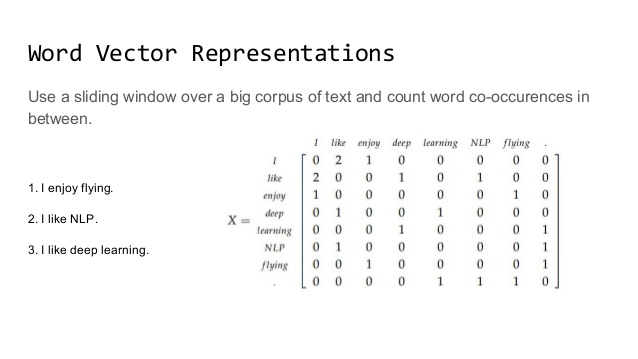
\includegraphics[width=0.5\textwidth]{figures/AFS/no1.jpg}}
\caption{Gambar Vektorisasi Kata.}
\label{no1}
\end{figure}

\item Jelaskan mengapa dimensi dari vektor dataset google bisa sampai 300. Dilengkapi dengan ilustrasi atau Gambar
\par Masing-masing nilai dalam vektor 300 dimensi yang terkait dalam sebua kata "dioptimalkan" dalam  beberapa hal untuk menangkap aspek yang  berbeda dari makna dan penggunaan kata itu.Dengan kata lain masing-masing dari 300 nilai sesuai dengan beberapa fitur abstrak kata. Menghapus kombinasi nilai-nilai ini secara acak akan menghasilkan vektor yang mungkin kurang informasi penting tentang kata tersebut dan mungkin tidak lagi berfungsi sebagai representasi yang baik dari kata itu. Atau singkat cerita mungkin ada lebih dari 3 miliar kata-kata dan kalimat atau data yang tidak mungkin disimpan dalam 1 diemensi vektor makan disimpan menjadi 300 dimensi vektor untuk mengurangi kegagalan memori.  Ilustrasinya bisa dilihat pada gambar berikut   \ref{no2}.
\begin{figure}[ht]
\centerline{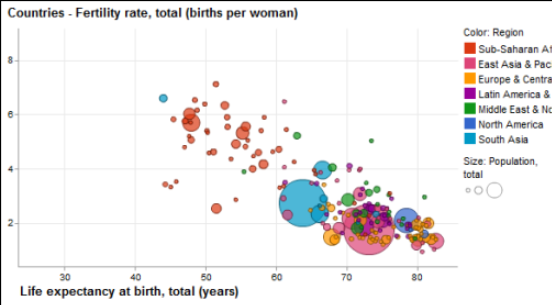
\includegraphics[width=0.5\textwidth]{figures/AFS/no2.png}}
\caption{Gambar Vektorisasi Dataset Google.}
\label{no2}
\end{figure}

\item Jelaskan konsep vektorisasi untuk kata. Dilengkapi dengan ilustrasi atau Gambar
\par Konsep untuk vektorisasi kata sebenarnya sama dengan ketika dilakukan input suatu kata pada mesin pencarian. Kemudian untuk hasilnya akan mengeluarkan ( berupa ) referensi mengenai kata tersebut. Jadi data kata tersebut didapatkan dari hasil pengolahan pada kalimat-kalimat sebelumnya yang telah diolah. Contoh sederhananya pada kalimat berikut ( Please click the alarm icon for more notifications about my channel ), pada kalimat tersebut terdapat konteks yakni channel, kata tersebut akan dijadikan data latih untuk mesin yang akan dipelajari dan diproses. Jadi ketika kita inputkan kta channel, maka mesin akan menampilkan keterkaitannya dengan kata tersebut sehingga akan lebih efisien dan lebih mudah.  Ilustrasinya bisa dilihat pada gambar berikut  \ref{no3}.
\begin{figure}[ht]
\centerline{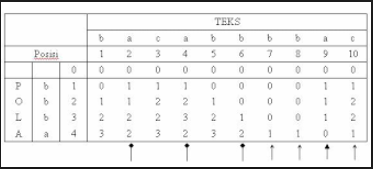
\includegraphics[width=0.5\textwidth]{figures/AFS/no3.png}}
\caption{Gambari Vektorisasi Kata.}
\label{no3}
\end{figure}

\item Jelaskan konesep vektorisasai untuk dokumen. Dilengkapi dengan ilustrasi atau Gambar
\par Vektorisasi Dokumen sebenarnya terbilang sama dengan konsep vektorisasi kata, hanya yang membedakan pada proses awalnya ( pada eksekusi awal ). Untuk vektorisasi dokumen ini, mesin akan membaca semua kalimat yang terdapat pada dokumen tersebut, kemudian kalimat yang terdapat pada dokumen tersebut akan di pecah menjadi kata-kata. Ilustrasinya bisa dilihat pada gambar berikut  \ref{no4}.
\begin{figure}[ht]
\centerline{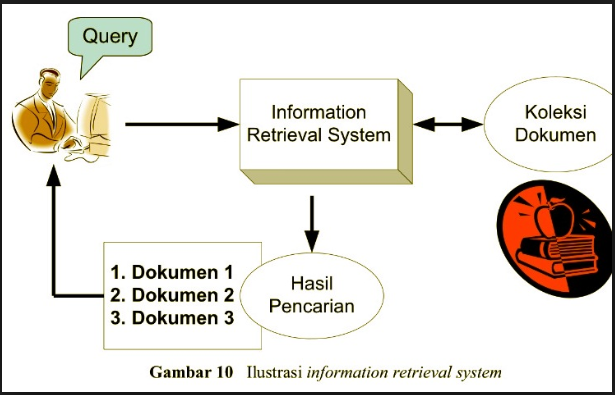
\includegraphics[width=0.5\textwidth]{figures/AFS/no4.png}}
\caption{Gambar Vektorisasi Dokumen.}
\label{no4}
\end{figure}

\item Jelaskan apa mean dan standar deviasi. Dilengkapi dengan ilustrasi atau Gambar
\par Mean adalah teknik penjelasan kelompok yang didasarkan atas nilai rata-rata dari kelompok tersebut. Rata-Rata (mean) ini didapat dengan menjumlahkan data seluruh individu dalam kelompok itu, kemudian dibagi dengan jumlah individu yang ada pada kelompok tersebut. \ref{no5m}
\begin{figure}[ht]
\centerline{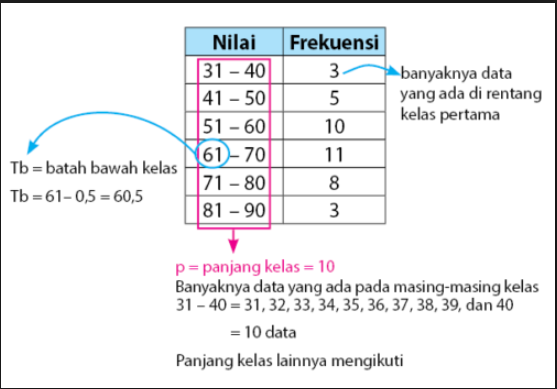
\includegraphics[width=0.5\textwidth]{figures/AFS/no5m.png}}
\caption{Gambar Mean.}
\label{no5m}
\end{figure}

\par Untuk standar deviasi sendiri merupakan sebuah teknik statistik yang digunakan dalam menjelaskan homogenitas kelompok ataupun dapat diartikan dengan nilai statistik dimana dimanfaatkan untuk menentukan bagaimana sebaran data dalam sampel, serta seberapa dekat titik data individu ke mean atau rata-rata nilai sampel yang ada. Ilustrasinya bisa dilihat pada gambar berikut  \ref{no5d}
\begin{figure}[ht]
\centerline{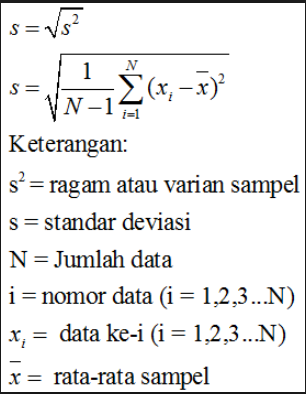
\includegraphics[width=0.5\textwidth]{figures/AFS/no5d.png}}
\caption{Gambar Deviasi.}
\label{no5d}
\end{figure}

\item Jelaskan apa itu skip-gram. Dilengkapi dengan ilustrasi atau Gambar
\par Skip-Gram mencoba memprediksi vektor kata-kata yang ada di konteks diberikan vektor kata tertentu. Skip-Gram membuat sepasang kata target dan konteks sebagai sebuah instance sehingga Skip-Gram cenderung lebih baik ketika ukuran corpus sangat besar.  Ilustrasinya bisa dilihat pada gambar berikut  \ref{no6}.
\begin{figure}[ht]
\centerline{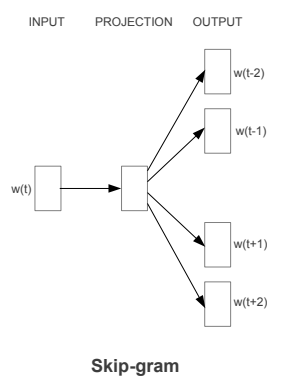
\includegraphics[width=0.5\textwidth]{figures/AFS/no6.png}}
\caption{Gambar Skip-Gram.}
\label{no6}
\end{figure}

\end{enumerate}